\chapter{The Uncertainty Principle}
  \section{The uncertainty principle for the free particle}
  
  In the previous lecture, we have derived the expression for the wavefunction of the free particle, for a Gaussian momentum wavefunction with width $ \sigma$ it is given by:
  \begin{equation}
  \psi(x,t) = \int _ {-\infty} ^{+\infty } dp \; e^{ - \frac{p^2 t}{2m \hbar}} \; \frac{e ^{ -\frac{\sigma ^2}{\hbar ^2}( p-p_0)^2} }{(\frac{2\pi \hbar ^2}{4 \sigma^2})^{1/2}} \; \frac{e^{ ipx/\hbar}}{\sqrt{h}}
  \end{equation}
  This integral is a Gaussian itself. Nevertheless, the width of the position Gaussian is inversely proportional to the momentum one, in particular :
  \begin{equation}
  \sigma(x) \sigma(p) \sim \hbar 
  \end{equation}
  This is a form of the celebrated uncertainty relation for position and momentum, which is directly derived from solving the free particle problem.
  \begin{figure} [h!]
  	\centering 
  	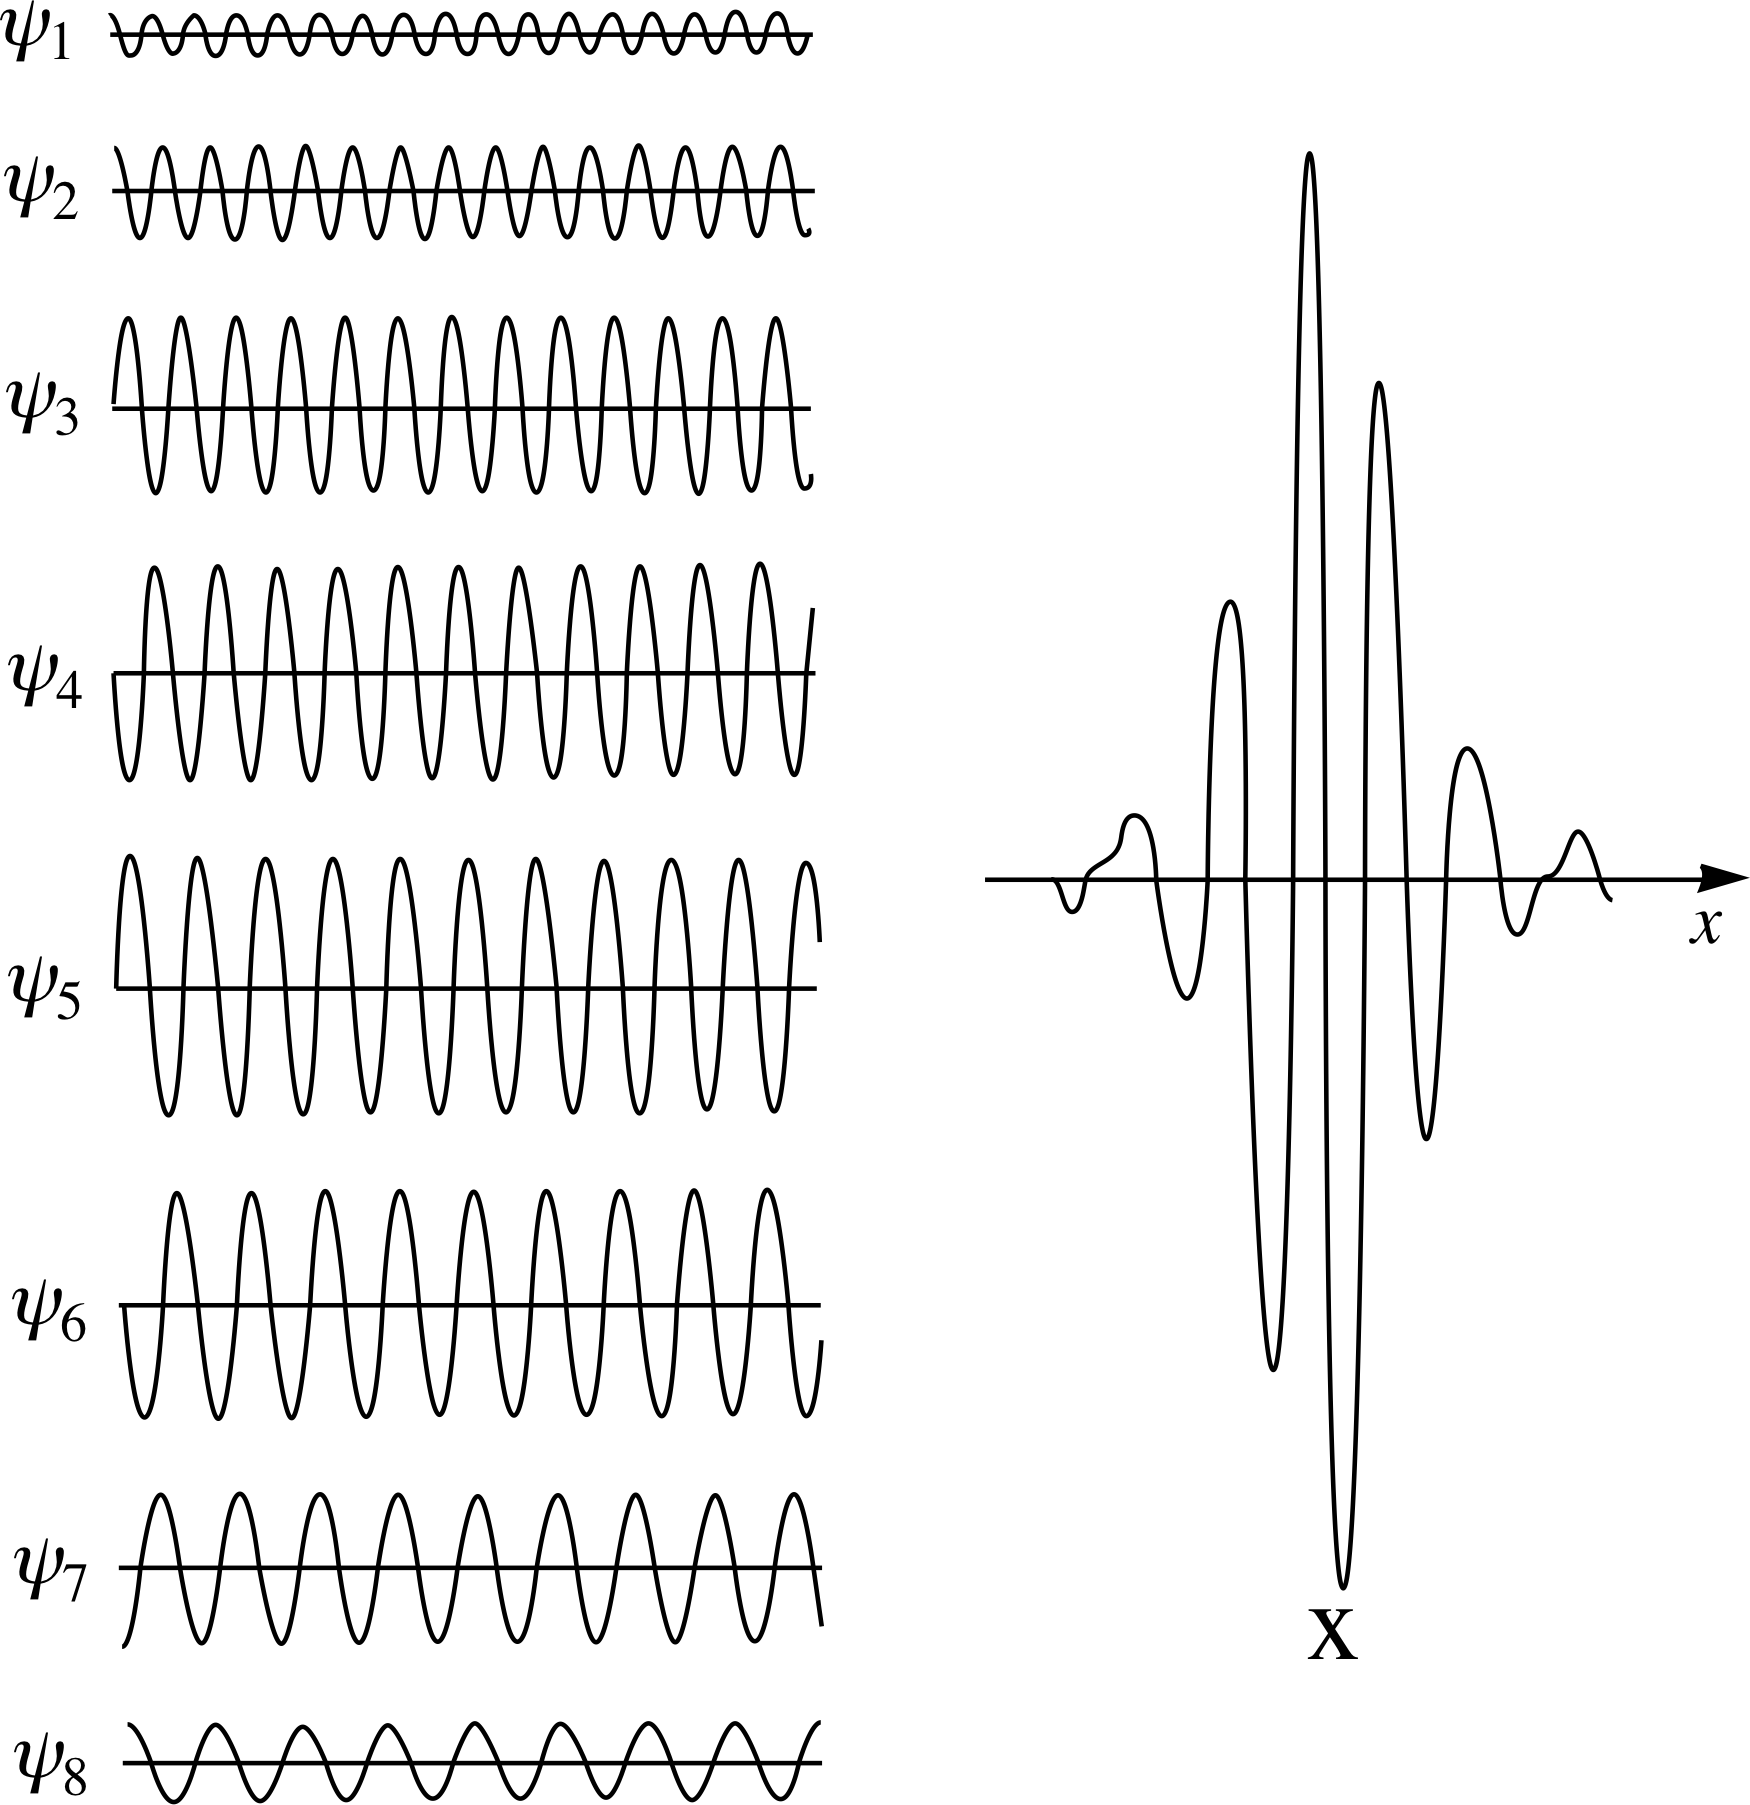
\includegraphics[scale = 0.7] {./figures/un}
  	\caption{ The position wavefunction is made from interference of infinite number of momentum wavefunctions}
  	\label{inter}
  \end{figure}
  The physical meaning for this relation is that in order to have a well-defined position for the wave-packet ( sharp width), we need to \textit{superimpose}  wide momentum wavefunctions ; and vice versa ( figure \ref{inter}). Implying the impossibility for having an absolute accurate measurement for either momentum and position regardless of the 'apparatus' used. Moreover, the increase in the accuracy in one implies the decrease in the other quantity.\\ \footnote{ The uncertainty principle is a fundamental property in nature unrelated to our methods of measurement}
  This principle is what -alone- explains the stability of atoms, counter to what the classical theory of electrodynamics predicts \footnote{In classical electrodynamics, an accelerating charge emits electromagnetic radiation}. Because electrons are bound within the atomic radius $ \sim 1$ \AA  They have to possess a velocity uncertainty of  about $ \sim 3 \times 10^3$ m/s or few eV c$ ^2$  of energy. For the electron to fall into the nucleus, i.e. being bound by the nuclear radius  $ \sim 10^{-5}$ \AA; it requires an enormous energy $ \sim 22$ MeV or more. Thus, electrons are forbidden from falling into the nucleus. Figure \ref{h} shows how the uncertainty principle, and schr\"{o}dinger's equation agrees completely with nature, the picture illustrates a real hydrogen atom's electron wavefunction indicating the probability of finding the electron in the vicinity of the atom.
  \begin{figure} 
  	\centering 
  	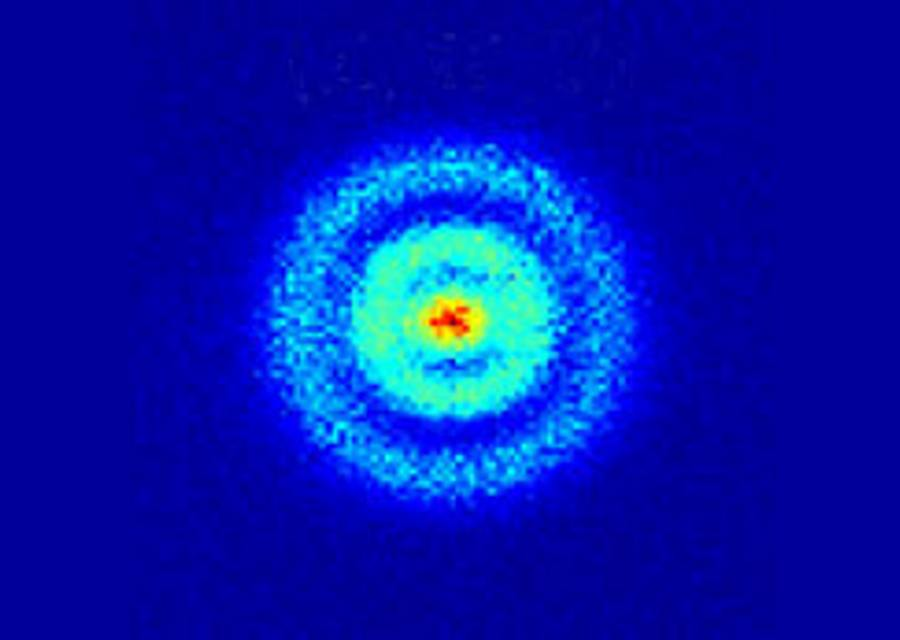
\includegraphics[scale = 0.2] {./figures/hatom.jpg}
  	\caption{ A real picture of Hydrogen atom; taken by special techniques. Indicating the probability of electron's position around the nucleus, in complete agreement with quantum theory. Reference:Stodolna, A. S., et al. Phys. Rev. lett. 110.21 (2013)}
  	\label{h}
  \end{figure}
  \section{General uncertainty principle}
  We can show - mathematically- a more general form of the uncertainty principle for position and momentum starting from the axioms of quantum mechanics; in particular the canonical commutation relation. 
  We start by defining the variance of an operator $ Var(A)$ \footnote{ We shal drop the 'hat' whenever it is understood we are talking about an operator} , as :
  \begin{equation}
  Var(A) = |(A- \langle A\rangle)^2| = \sigma(A)^2
  \end{equation}
  In the position representation this equals to $ \int dx \psi^*  \sigma(A)^2 \psi $. We define the \textbf{Schwartz inequality }:
  \begin{equation}
  |A|^2 | B|^2 \geq | AB| ^2
  \end{equation}
  For $ A = \sigma(X)$ and $ B= \sigma(P)$; we have :
  \begin{equation}
  Var(X)\; Var(P) = | \langle X\; P \rangle | ^2
  \label{unse}
  \end{equation}
  But the product $ XP$ can be expressed as :
  \begin{equation}
  XP =  \frac{1}{2}\,[ X, P]\; +\;\frac{1}{2} \left( X\,P\;+\;P\,X\right) 
  \end{equation}
 
  \begin{mdframed}
  	Proof :\\
  	Start by Writing :
  	\[
  	XP = XP - \frac{1}{2} PX + \frac{1}{2} XP
  	\]
  	Moreover :
  	\[
  	XP = \frac{1}{2} PX + \frac{1}{2} XP - \frac{1}{2} PX + \frac{1}{2} XP
  	\]
  	Gathering terms, we obtain :
  	\[
  	XP =  \frac{1}{2}[ X, P] +\frac{1}{2} ( XP+PX) \; \; \; \; \; \Box
  	\]
  \end{mdframed}
  Substituting this result in \eqref{unse}; and knowing $ [ X, P]= i \hbar$ we obtain:
  \begin{equation}
  Var(X )b \; Var(P) \geq |\frac{1}{2} i\hbar| ^2 +  \frac{1}{4} | (\langle PX\rangle) +\langle XP\rangle | ^2 
  \end{equation}
  Since both $\langle PX\rangle$ and $\langle XP\rangle$ are equal, and the expression $ \frac{1}{4} | (\langle PX\rangle) +\langle XP\rangle | ^2 $ is non-negative . We may write:
  
  \begin{equation}
  Var(X) \; Var(P) \geq \frac{\hbar ^2}{4}
  \end{equation}
  Taking the square root :
  \begin{equation}
  \boxed {\sigma(X) \sigma(P) \geq \frac{\hbar}{2} }
  \end{equation}
  In fact, this result can be generalised for any two non-compatible observables $A$ and $B$:
  \begin{equation}
  \boxed {\sigma(A) \sigma(B) \geq \frac{1}{2} |\langle [ A, B]\rangle |}
  \end{equation}
  This is the general form of uncertainty principle. 
  \section{Uncertainty in time and energy}
  In modern physics, we were introduced to the \textbf{quantum harmonic oscillator.} Although we shall revisit it soon, but we may recall an import result. Which is the\textbf{ zero-point energy}:
  \begin{equation}
  E_0 = \frac{1}{2} \hbar \omega
  \label{osc}
  \end{equation}
  Although the harmonic oscillator is in its ground state, yet it has an amount of energy inversely proportional to its period of oscillation. If the period is dependent of  measurement - like any quantum mechanical observable- to assign the period with accuracy, we need to measure time with precision. This implies a large $ \omega$ of the oscillator that should be used for measurement since $T \propto  \frac{1}{\omega}$. That implies adding a lot of energy to the system - even if it was in the ground state- by the above equation \eqref{osc}. In fact this translates to :
  \begin{equation}
  \boxed{ \sigma (E) \sigma (t) \geq \frac{\hbar}{2}}
  \end{equation}
  This principle holds for any quantum system, not just the harmonic oscillator. However, it is easier to see in this case. \\
  The time-energy uncertainty principle has rather deep implications, in particular for the law of energy conservation. One can 'trade' energy with time, by adding energy -from nothing- to the system provided it is for short period of time. This is an important phenomena observed a lot in particle physics. For example the \textit{weak interaction } which allow beta radiation ( neutrons decaying into protons or vice versa). A particle called W- boson , having about 80 times the mass of proton is created from nothing, but for a very short time $ \sim 10^{-18}$ sec. Just enough to allow the weak interaction to occur.
  \begin{figure}
  	\centering
  	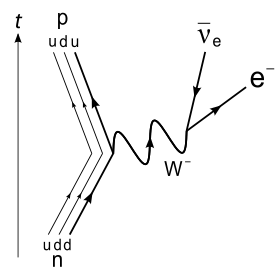
\includegraphics[ scale= 0.5]{./figures/weak}
  	\caption{ A diagram showing the weak interaction mediated by the W boson which is created from nothing by the uncertainty principle} 
  \end{figure}  
  \section{ Ehrenfest theorem}
  As we have seen, classical mechanics is obtained from averaging quantum mechanical results. For example the conservation of energy is an average result from the uncertainty principle discussed above. Therefore, we need to prove that from  quantum mechanics we can arrive to classical equations of motion. This is \textbf{Ehrenfest theorem}. \\
  The classical observable $ \omega$ is the expected-value of the quantum mechanical operator $ \hat{\Omega}$:
  \begin{equation}
  \omega = \langle \hat{ \Omega} \rangle = \langle \psi | \hat{\Omega}| \psi \rangle 
  \end{equation} 
  Let's take the time derivative of the expected-value $d/dt (\langle \hat{ \Omega} \rangle )$:
  \[
  \frac{d}{dt}\left( \langle \psi | \hat{\Omega}| \psi \rangle \right) 
  \]
  by the product rule:
  \[
  \frac{ \rd \langle \psi |}{\rd t} \hat{\Omega} | \psi \rangle + \langle \psi | \frac{\rd\hat{\Omega}}{\rd t} | \psi \rangle + \langle \psi | \hat{\Omega} \frac{\rd | \psi \rangle}{\rd t}
  \]
  Now by substituting in Schr\"{e}dinger's equation $  \frac{1}{i \hbar} \hat{H} | \psi \rangle =\frac{\rd | \psi \rangle}{\rd t}$, and its complex conjugate. We obtain :
  \[
  \frac{d}{dt}\left( \langle \psi | \hat{\Omega}| \psi \rangle \right)  =
  - \frac{1}{i \hbar} \langle \psi| \hat{H} \hat{\Omega} | \psi \rangle + \langle \psi | \frac{\rd\hat{\Omega}}{\rd t} | \psi \rangle + \frac{1}{i \hbar}  \langle \psi | \hat{\Omega} \hat{H} | \psi \rangle
  \]
  This is equivalent to :
  \begin{equation}
  \boxed{
  	\frac{d}{dt}\left(\langle \hat{\Omega} \rangle\right)  = \frac{1}{i\hbar} \langle [ \hat{\Omega}, \hat{H}]\rangle + \langle\dfrac{\partial \hat{\Omega}}{\partial t }\rangle
  }
  \end{equation}
  This is the exact mathematical formula for Ehrenfest theorem.
  Now, we turn to applying this theorem to the operators $ p$ and $ X $, in order to recover the classical equations of motion:
  \[
  \dot{\langle p\rangle }  = \frac{1}{i \hbar} \langle [p, V(x)]\rangle
  \]
  since $p$ is time-independent, and the Hamiltonian takes the form : $ H = \frac{p^2}{2m} +V$.\\
  Working in the position representation, the above commutator is written explicitly as :
  \[
  - \int dx \psi ^* \dfrac{\rd}{\rd x}\left( V \psi\right) + \int dx \psi ^* V \dfrac{\rd}{\rd x}\left( \psi \right) 
  \]
  Applying the product rule to the first expression :
  \[
  - \int dx \psi ^* \dfrac{\rd}{\rd x}\left( V \right)  \psi - \int dx \psi ^* V \dfrac{\rd}{\rd x}\left( \psi \right)  + \int dx \psi ^* V \dfrac{\rd}{\rd x}\left( \psi \right) 
  \]
  Thus we get:
  \begin{equation}
  \dot{\langle p\rangle }  = - \langle  \dfrac{\rd V}{\rd x}  \rangle
  \end{equation}
  Which is Newton's second law, or one of Hamilton's equations ( recall that $ F= - \frac{ d V}{dx}$)
  \begin{equation}
  \boxed{
  	\langle [ p, H]\rangle = - \langle  \dfrac{\rd V}{\rd x}  \rangle
  }
  \end{equation}
  Let's now apply Ehrenfest theorem. to the position operator $X$:
  \[
  \dot{\langle X \rangle } = \frac{1}{i \hbar} \langle [ X, \frac{p^2}{2m}]\rangle
  \]
  since $X$ is also time-independent, and the potential is only a function of position. We need to use the result from lecture (3), equation (22) 
  \[
  [A, f(B)] = [ A, B] \frac{ d f(B)}{dB}
  \]
  with $ A = X$,  $ B = p$ and $ f(p) = p^2$; we obtain:
  \[
  \dot{\langle X \rangle } = \frac{1}{2i m \hbar} \langle [ X, p] \frac{d}{dp} ( p^2)\rangle
  \]
  $\Leftrightarrow $
  \[
  = \frac{1}{2 i m \hbar} ( i\hbar) (2 \langle p \rangle)
  \]
  Finally :
  \begin{equation}
  \dot{\langle X \rangle } = \frac{1}{m} \langle p \rangle
  \end{equation}
  The definition for the classical velocity, or the second Hamilton's equation:
  \begin{equation}
  \boxed{
  	\langle [ X, H]\rangle = \frac{1}{m} \langle p \rangle
  }
  \end{equation}
  
  \section{Problems}
  \begin{enumerate}
  	\item We define the \textbf{first ionisation energy }, as the energy needed to free an electron from the vicinity of its atom. For Carbon 14, it is found; by detailed quantum mechanical calculations and experimental verification that the first ionisation energy is $ E_{min} = 11.3$ eV.
  	\begin{enumerate}
  		\item Estimate using the uncertainty principle $ E_{min}$, if you know the electron in the C(14) atom is confined to a box of $ x= 0.182$ nm. and $ E= p^2/ 2m$ 
  		\item Provide an explanation, from the uncertainty principle for not observing 'protons' being confined to atoms; use the last calculations on C(14) as a guide.
  	\end{enumerate}
  	\begin{figure}[h!]
  		\centering
  		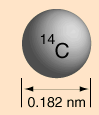
\includegraphics[scale= 0.6]{./figures/c_atom}
  	\end{figure}
  	\item 	What is the origin of electrons in beta decay ?\\
  	Beta ($\beta^-$) decay is a nuclear decay process that turn a neutron into a proton. This happens when the number of neutrons are imbalanced, hence the nucleus decays by emitting an electron and another particle called the  anti-neutrino in order to be stable.\\ In the early days of nuclear physics, and because of the beta decay, it was argued that the nucleus is composed of electrons and protons. Thus electrons emitted in the beta decay are bound in the nucleus. This is known as the proton-electron hypothesis.\\ Provide an argument against this hypothesis from the uncertainty principle. Take the C(14) decay into N(14) as an example. The nuclear radius for C(14) is $ 5.8 \times 10^{-15} $m and the energy of the emitted electron is at maximum $ E_{max} = 0.016$ MeV. 	
  	\begin{figure}[h!]
  		\centering
  		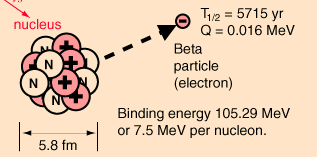
\includegraphics[scale= 0.6]{./figures/decay}
  	\end{figure}
  	\item Einstein's Recoiling Slit Experiment.\\
  	Einstein was known for his opposition against the quantum theory, although he admitted its validity. One of the arguments Einstein has made against the quantum theory - in particular the uncertainty principle- is a 'modified' version of the double-slit experiment . This full thought experiment is constructed as the figure shows.
  	\begin{figure}[h!]
  		\centering
  		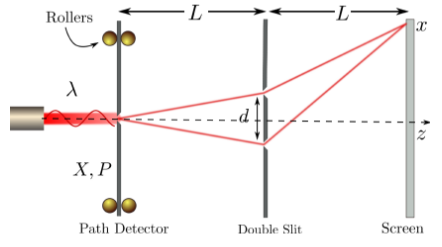
\includegraphics[scale= 0.4]{./figures/ese}
  	\end{figure}
  	However, we shall take a simpler one. The experiment goes as follows :\\
  	Imagine having a narrow slit, with small width $ d$, a quantum particle passes though this slit . This let us \textit{detect}  its position by $ d$, as a result, this causes a momentum uncertainty of $ \sim \frac{\hbar}{2 d}$. However, Einstein suggested that we can measure the particle's momentum from the recoil of the screen of which the particle collides with after passing through the slit. If the screen is free to move in the $ x$ direction, by the laws of momentum conservation, the recoil of the screen is related to the incident particle momentum. In fact, the extended version of this thought experiment is done experimentally cf.(Nature Photonics 9, 120–125 (2015)).\\
  	Of course, Einstein has missed something in his thought experiment. Niels B\"{o}hr had provided an answer to Einstein's experiment defending the uncertainty principle. Can you guess what was that argument ?
  	
  	\item Prove Ehrenfest theorem in Heisenberg picture.
  \end{enumerate}
  (pictures are from Hyperphysics website, \url{http://hyperphysics.phy-astr.gsu.edu/hbase/hframe.html})